% MFP: A patcher extensible in Python and Faust
% Copyright (c) 2025 Bill Gribble <grib@billgribble.com>

% To generate the correct references using BibTeX, run
%     latex, bibtex, latex, latex

% 1) Please compile using latex or pdflatex.
% 2) If using pdflatex, you need your figures in a file format other than eps! e.g. png or jpg is working
% 3) Please use "paperftitle" and "pdfauthor" definitions below

%------------------------------------------------------------------------------------------
%  !  !  !  !  !  !  !  !  !  !  !  ! user defined variables  !  !  !  !  !  !  !  !  !  !  !  !  !  !
% Please use these commands to define title and author(s) of the paper:
\def\papertitle{MFP: A graphical patcher extensible in Python and Faust}
\def\paperauthorA{Bill Gribble}
\def\paperauthorB{}
\def\paperauthorC{}
\def\paperauthorD{}

% Authors' affiliations have to be set below

%------------------------------------------------------------------------------------------
\documentclass[a4paper]{article}

\usepackage{LAC-25}
\usepackage[margin=2cm]{geometry}
\usepackage{amsmath,amssymb,amsfonts,amsthm}
\usepackage{euscript}
\usepackage[utf8]{inputenc}
\usepackage[T1]{fontenc}
\usepackage{ifpdf}
\usepackage{color}
\usepackage{listings}
\definecolor{mygrey}{rgb}{0.96,0.96,0.96}
\lstset{
  tabsize=4,
  basicstyle=\ttfamily,
  backgroundcolor=\color{mygrey},
  captionpos=b,
  breaklines=true
}

\usepackage[english]{babel}
\usepackage{caption}
\usepackage{subfig, color}

\setcounter{page}{1}
\ninept

\usepackage{times}
% Saves a lot of ouptut space in PDF... after conversion with the distiller
% Delete if you cannot get PS fonts working on your system.

\def\:{\hskip0pt}

% pdf-tex settings: detect automatically if run by latex or pdflatex
\newif\ifpdf
\ifx\pdfoutput\relax
\else
   \ifcase\pdfoutput
      \pdffalse
   \else
      \pdftrue
\fi

\ifpdf % compiling with pdflatex
  \usepackage[pdftex,
    pdftitle={\papertitle},
    pdfauthor={\paperauthorA, \paperauthorB, \paperauthorC, \paperauthorD},
    colorlinks=false, % links are activated as colror boxes instead of color text
    bookmarksnumbered, % use section numbers with bookmarks
    pdfstartview=XYZ % start with zoom=100% instead of full screen; especially useful if working with a big screen :-)
  ]{hyperref}
  \pdfcompresslevel=9
  \usepackage[pdftex]{graphicx}
  \usepackage[figure,table]{hypcap}
\else % compiling with latex
  \usepackage[dvips]{epsfig,graphicx}
  \usepackage[dvips,
    colorlinks=false, % no color links
    bookmarksnumbered, % use section numbers with bookmarks
    pdfstartview=XYZ % start with zoom=100% instead of full screen
  ]{hyperref}
  % hyperrefs are active in the pdf file after conversion
  \usepackage[figure,table]{hypcap}
\fi

\title{\papertitle}

\affiliation{ \paperauthorA}
{{\tt \href{mailto:grib@billgribble.com}{grib@billgribble.com}}}

\begin{document}

% more pdf-tex settings:
\ifpdf % used graphic file format for pdflatex
  \DeclareGraphicsExtensions{.png,.jpg,.pdf}
\else  % used graphic file format for latex
  \DeclareGraphicsExtensions{.eps}
\fi

\maketitle

\begin{abstract}
MFP is a graphical patching system distinguished by the ready
availability of Python data types and operations in patches.
Recent work has added support for live coding of
message\:-\:processing patch elements in Python, and of
signal\:-\:processing patch elements in Faust.  Its extensibility
and rich set of message data types give MFP some nice
capabilities for interactive patching.
\end{abstract}

\section{Introduction}
\label{sec:intro}

My first exposure to live coding for audio was Pure Data (Pd)
\cite{Puck:PureData}. As a programmer, I have always loved the
read-eval-print loop (REPL) as a way of exploring solutions and
incrementally building and running code. Pd's interface
immediately connected to the part of my brain that likes REPL
development. It's such a great way of experimenting, testing,
and, once you get something going, improvising and performing on
a patch that just keeps running even when you make mistakes.

The original development of MFP was inspired by the realization
that a dataflow patcher's "REPL" really is just code, expressed
in an unconventional form. I know this isn't exactly a stroke of
genius -- one of the mottos of Pd is "the diagram is the
program", so it's basically printed on the tin. What was
interesting to me was looking at what it means for a graphical
patcher to be a programming language. How do the concepts of a
conventional programming language map onto the expressive
vocabulary of a patch? Are there gaps in the correspondence that
can lead to insights towards better patching systems? Can the
expressive power of the implementation language give a boost to
the patcher? Can the need for real-time performance be reconciled
with a rich and dynamic data model?

When regarded as programming languages, dataflow patchers have
many aspects that connect them to the programming language
"family tree".  They are somewhat like functional languages,
in that values are returned from functions and marshaled into
parameter lists of other functions without resorting to variable
names or side effects.  Message passing, the main mechanism
patchers use for data interchange and code invocation, goes back
to Smalltalk and beyond. Patchers support modular programming
via the ability to start with simple units and compose them to
make more complex behavior. They have a variety of data types,
input/output mechanisms, and modes of interaction with the wider
system. So it's reasonable to expect patching languages to
support a pretty wide variety of usual programming paradigms and
patterns.

However, when I started trying to make more complex patch\-es in
Pd, especially ones that leaned into the manipulation of
non\:-\:audio data, I quickly ran into frustrations with the data
model that made it quite difficult to do things that should (in
my opinion) have been simple. I wondered if breaking out of the
space\:-\:delimited textual syntax and limited type\:-\:vocabulary of Pd
objects, and using the data types from a dynamic language such as
Python instead, could give a graphical patcher more of the power
of a full programming language.

The result of my explorations is MFP. The patch editor and
message processing engine are implemented in Python and directly
expose the Python data model, library, and evaluator to the user.
The real\:-\:time audio engine is implemented in C and is loosely
coupled to the UI and message\:-\:processing system via an RPC
mechanism. The overall experience is similar to Pd or Max/MSP,
but there has been no attempt at compatibility.

When I presented it at the 2013 edition of LAC
\cite{Gribble:2013}, MFP was functional enough and interesting
enough that I thought it was worth continuing to develop. Now,
some 12 years later, it has evolved in various foreseen and
unforeseen directions and is, I think, worthy of a
re\:-\:introduction to the Linux audio community.


\section{What is it?}

My vision for MFP is as a multitool for REPL\:-\:style incremental
development that can fit in to music composition, performance,
and recording workflows wherever some bespoke functionality is
needed.

In operation, MFP will look pretty familiar to users of Pd or
Max/MSP. See Figure~\ref{fig:appview} for a sample session. Its
interface allows the user to interactively build {\it patches},
which are sets of directed graphs of {\it processors}. A
processor has a set of inputs, which handle either {\it messages}
(discrete pieces of data of any type) or {\it signals} (streams
of floating-point audio data). It produces outputs which are
likewise either messages or signals. The behavior of a processor
is determined from a type-name and arguments provided at
creation. The type-name can resolve to either a builtin MFP
processor type, of which there are over 150, a user-created
patch, or an arbitrary Python callable.

In the patch editing window, processors can appear as plain
boxes, or can have a variety of visual representations that allow
for patch control or feedback: message boxes, number boxes,
buttons, sliders, dials, X/Y plots, text with Markdown
formatting. Patches used as building blocks by other patches can
export a UI of their choice to appear on their placeholder in the
containing patch. Direct connections between processor nodes are
represented by lines.

Named message and signal buses, comparable to Pd's {\tt [s]} and
{\tt [r]}, appear as dots terminating connection lines, called {\it
vias}. Names and scoping are an important part of MFP, and vias
represent one of the main user-visible aspects of naming: each
via is paired with its companion(s) by a name, visible in the UI,
that must be resolved to find the intended connection-partner.

The patch as a whole is modeled as a stack of {\it layers}, which
are something like Pd {\it subpatches}: they are primarily a
visual organizational tool to reduce clutter in the patching
interface. One layer of a patch is visible at a time. Multiple
patches can be displayed simultaneously, using a multi-page tiled
workspace manager.

The nomenclature of {\it layers} and {\it vias} comes from
electronics design, where a printed circuit board is made up of a
multi-layer sandwich of conductive and nonconductive material. To
me, a dataflow patch looks a bit like a circuit board populated
with chips and other components. A {\it via} is a plated
conductive hole, effectively a wire, that connects from one layer
through to another. The visual representation of a via as a
dot/circle is intended to evoke that.

\begin{figure*}[ht]
\centerline{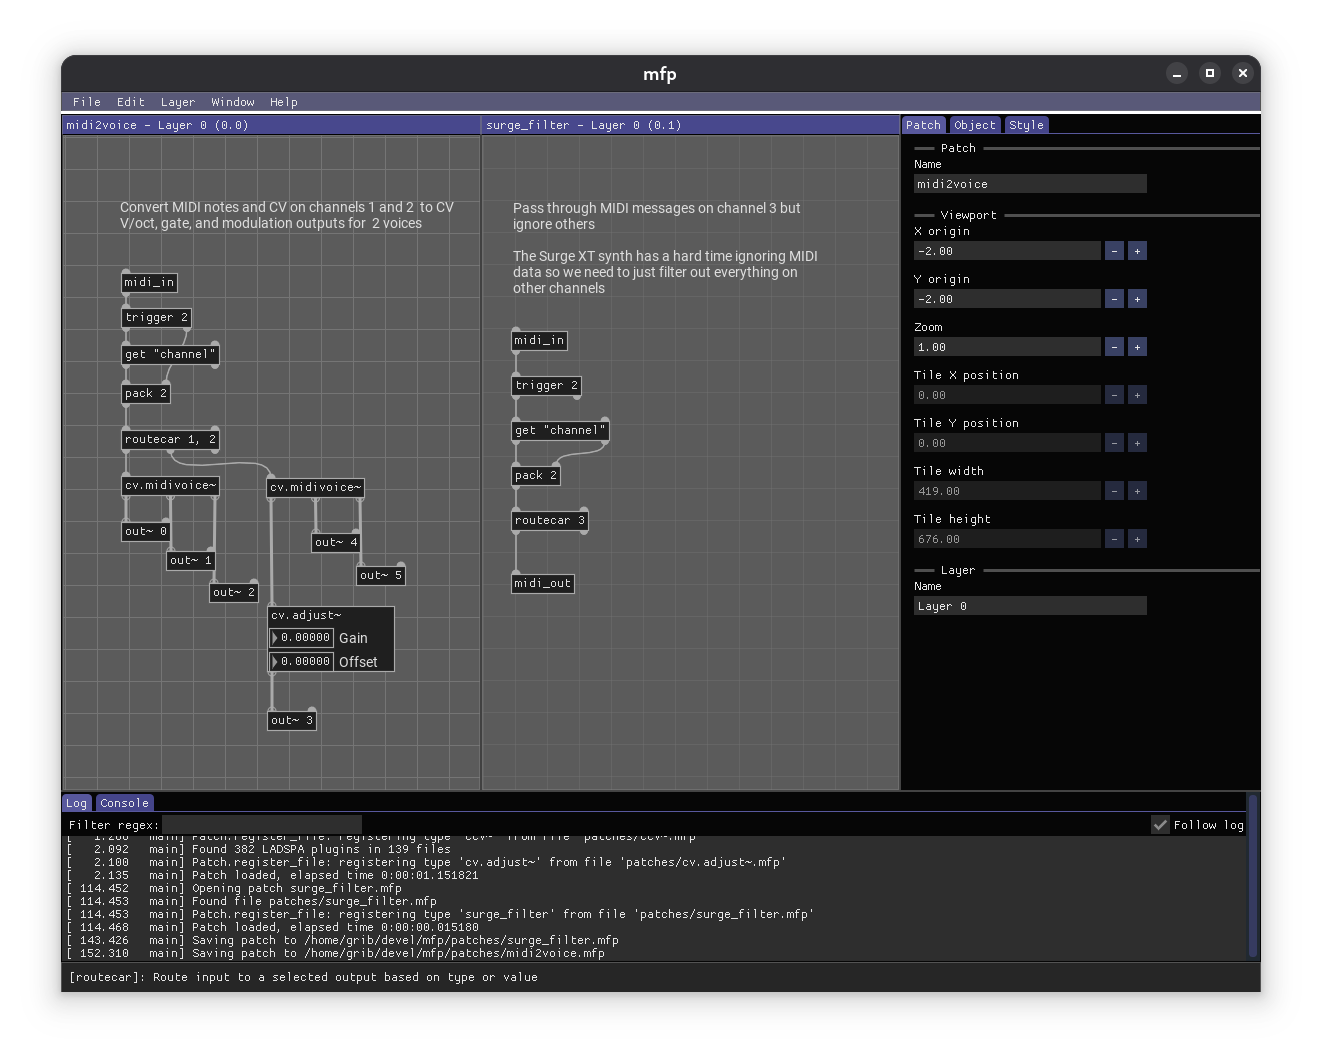
\includegraphics[width=6in]{appview.png}}
\caption{\label{fig:appview}{
    \it View of MFP app window, featuring tiled workspace,
    object info panel on the right, and log window with
    status/tooltip line below.
}}
\end{figure*}


\section{Capabilities}

An exhaustive listing of MFP's features would be quite long and
probably boring. Instead, I would like to highlight a curated set
of features that might be of interest when trying to decide if
you want to download MFP and give it a try.

\subsection{Data model}

Message data is plain Python objects of any type. Numbers,
strings, arrays, dictionaries, sets, custom classes, anything.
Literal data typed into the UI is evaluated as it would be in a
Python REPL. This means that message boxes and processor argument
lists can contain Python expressions to be evaluated at object
load time. See Figure~\ref{fig:datamodel} for some examples.

{\bf Partial application syntax.} A special syntax allows for
literals that represent partially-applied functions. When sent as
a message, {\tt @funcname([args], [kwargs])} will be consumed by its
first recipient and applied to the recipient as a method call.

{\bf Deferred evaluation syntax.} Another special syntax
extension allows for literals that are not evaluated until they
enter the processing network. A initial comma preceding an
expression will wrap it in a Python {\tt lambda} form that is not
called until the message is sent. This allows for time-varying
results from a "literal" message box.

\begin{figure}[ht]
\centerline{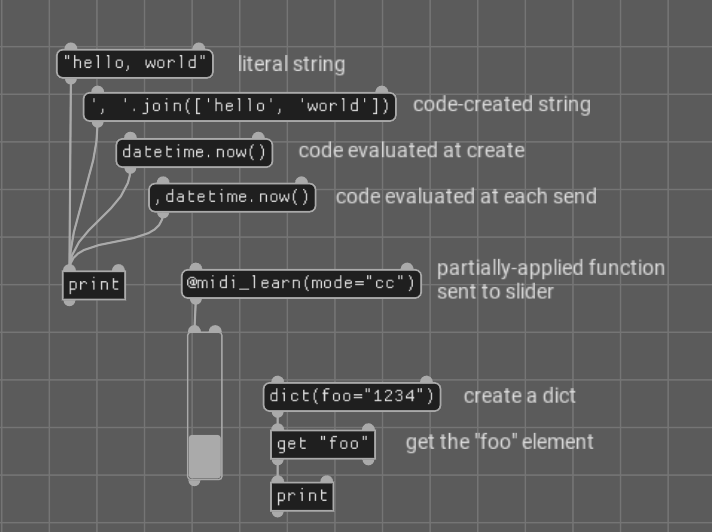
\includegraphics[width=3.25in]{datamodel.png}}
\caption{\label{fig:datamodel}{
    \it Patch fragments demonstrating features of the MFP data model,
    including vias, partial application, and deferred evaluation
}}
\end{figure}


\subsection{Python live-coding }

The message\:-\:passing system at the heart of MFP is implemented in
Python, and there are several pathways enabling the user to
access the standard Python library and/or write Python code
directly into the patching interface.

{\bf The {\tt func} processor.} {\tt [func]} is a very thin wrapper
around Python's {\tt lambda}. It allows you to write a single
Python expression directly in a processor box. The arity of the lambda
is extracted via Python's {\tt inspect}, and inlets are created for
each argument.

{\bf Library access.} Any callable Python object can be
automatically wrapped as a MFP processor element. If you create a
processor element called {\tt re.split}, which is not an MFP
builtin, it will look for a callable bound to that name. As with
{\tt func}, {\tt inspect} is used to find its argument signature
and create an object with the appropriate inputs.

{\bf Custom processor types.} This enables live coding of new
message processors in Python. To create a custom processor type
called {\tt myfunc}, we can attach the Python code to define a
function called {\tt myfunc} directly to the processor via its
"Custom code" parameter, and allow the autowrapping process to
discover it.

{\bf Offline coding.} A user\:-\:provided RC file, loaded at startup,
can define new data types and builtin processor types using MFP's
internal framework.

See Figure~\ref{fig:pythonlivecoding} for some examples of these
mechanisms in use.

\begin{figure}[ht]
\centerline{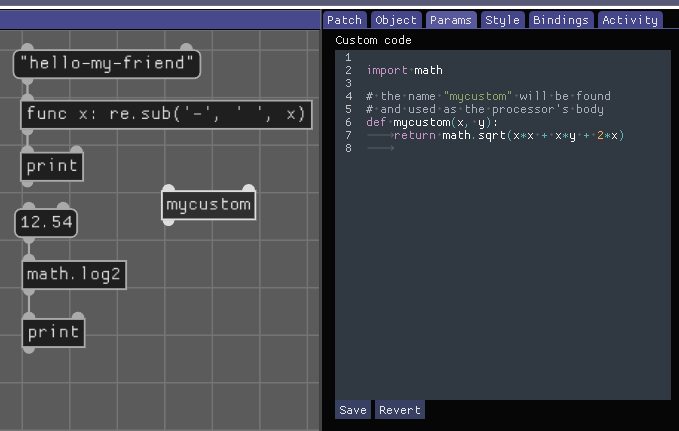
\includegraphics[width=3.25in]{python_livecoding.png}}
\caption{\label{fig:pythonlivecoding}{
    \it Several mechanisms for live-coding Python in MFP:
    [func], custom code, and automatically wrapped Python
    library functions
}}
\end{figure}

\subsection{Faust live-coding }

The {\tt [faust\textasciitilde]} object supports live coding of
DSP algorithms in Faust. Code can be typed directly into the UI
or loaded from files, and can be parameterized or customized via
Python at compile time.

This is possible via the "Custom code" parameter mentioned above.
The {\tt [faust\textasciitilde]} processor looks for a special
Python variable called {\tt faust\_code} in the custom code
block. This variable can be defined as a constant, literal string
(the Python triple\:-\:quote syntax works well to support a formatted
Faust program in a Python string), it can be the result of Python
file operations to load from a named file, or it can be assembled
by Python string formatting and manipulation operations.

Once compiled to LLVM within the {\tt mfpdsp} process, the Faust
DSP object is inspected to extract parameters and I/O channels so
that the processor element's input/output profile matches the
signature of the DSP code.

See Figure~\ref{fig:faustlivecoding} for how this looks in
practice.

\begin{figure}[ht]
\centerline{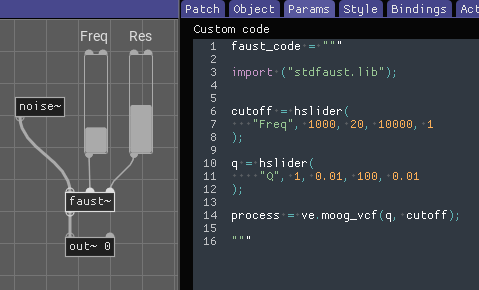
\includegraphics[width=3.25in]{faust_livecoding.png}}
\caption{\label{fig:faustlivecoding}{
    \it Live coding in Faust using the {\tt [faust\textasciitilde]} object
}}
\end{figure}


\subsection{Debugging}

Since MFP is still very much a work in progress, a lot of the
debugging functionality is built as much to debug MFP as it is to
debug user patches, but it's useful for both.

{\bf Python console.} There is an always\:-\:available Python console
that can directly access and manipulate the app's data.  For
example, the default patch that is created when you open MFP with
no arguments is {\tt app.patches['default']}

{\bf Breakpoints and step execution.} MFP supports step debugging
of patches with the {\tt [bp]} breakpoint setter. A message
encountering a {\tt [bp]} causes the Python console to enter a
simple debug mode, inspired by {\tt pdb}, which allows for direct
inspection of internal processor state and tracing of the
marshalling and dispatch process.

{\bf Snoop mode.} Enabling "snoop mode" on a connection briefly
displays any messages passing through the connection.

{\bf UI state inspector.} A UI state inspector, modeled after the
Redux devtools inspector, is provided by the Flopsy state
management library \cite{Gribble:Flopsy}. It allows for detailed
analysis of the time sequence of changes to the UI.

\subsection{MIDI and OSC}

Every element in a patch can be controlled with MIDI or OSC
messages.  MIDI and OSC events can be easily handled, created,
and sent within a patch.

{\bf MIDI message types.} A set of Python types representing the
various flavors of MIDI messages are available to patches: {\tt
NoteOn}, {\tt NoteOff}, {\tt MidiCC}, {\tt MidiPitchbend}, etc.
These types can be used to filter/route events by type with the
{\tt [route]} family processors. Fields are accessible using the
{\tt [get]} and {\tt [set!]} processors.

{\bf Automatic controls.} Every element has an OSC address and
can accept OSC messages. The "Bindings" tab of the processor info
display shows the currently active OSC routes and data types. OSC
messages to the displayed address will be sent to the leftmost
inlet of the targetted processor.

{\bf Learning controls.} To connect an external MIDI controller to
a processor, send the message {\tt @midi\_learn} to the processor or
choose "Learn MIDI controller" from the context menu.
The next MIDI events received will be analyzed and a filter and
value accessor will be determined from the properties of the event.

{\bf Explicit message handling.} The builtin processor types {\tt
[midi\_in]}, {\tt [midi\_out]}, {\tt [osc\_in]}, and {\tt
[osc\_out]} enable sending and receiving of MIDI and OSC messages
outside the automatic and learned controllers on specific
objects. Figure~\ref{fig:appview} shows some of these processors
in action.


\subsection{Plugin hosting}

The {\tt [plugin\textasciitilde]} object enables loading external
plugins as MFP DSP objects. Currently, only LADSPA plugins are
supported but LV2 and CLAP are planned.

The audio and control ports of the plugin are determined from the
LADSPA plugin descriptor and mapped to inlets and outlets on the
{\tt [plugin\textasciitilde]} processor.


\subsection{Patches as plugins}

An MFP patch can be saved as an LV2 plugin. There are limits on the
live editing that can be done (for example, the number of inputs and
outputs of the plugin are fixed at save time) but for the most part
the patch works as normal.

LV2 plugins exist as "bundles" which are (to simplify) a shared
library implementing the plugin, plus metadata, in the form of
the {\tt manifest.ttl} file (describing tha plugin) and any
additional plugin\:-\:specific metadata.

For an MFP patch, the shared library is the {\tt libmfpdsp.so}
library that implements the MFP DSP engine, and the
plugin\:-\:specific metadata includes the MFP patch save file. Since
the Python runtime is an essential part of patch loading and
operation, we need to make sure that it is loaded on plugin
initialization.

Normally, when MFP is launched, the Python "main" process is
launched first, and it forks the DSP engine and communicates with
it through a socket. The LV2 entry points in {\tt libmfpdsp.so}
reverse this process, forking the Python main process (if it is
not already running) in a mode that enables it to know what is
happening.

Since the Python runtime also manages the MFP UI, the management
of UI for the plugin is not currently left for the LV2 host to
control via the normal mechanism of the LV2 UI extension. Rather,
an "Edit" control added to the plugin causes the MFP graphical editor to
open the patch. This may change in the future.


\section{Implementation}

\subsection{Runtime components}

When running, MFP consists of several components working in concert.

\begin{itemize}
\item[]
{\bf mfpmain:} A Python program that is the primary execution
environment of MFP. It handles the processing of discrete
message data, delegating all real\:-\:time signal processing to the
mfpdsp process.

\item[]
{\bf mfpgui:} A Python program that implements the UI. It currently
supports 2 backends: the original Clutter/Gtk UI and a newer one
built with Dear ImGui.

\item[]
{\bf mfpdsp:} A C program that implements the DSP engine and JACK
client interface.
\end{itemize}

These three are loosely coupled, communicating via an
asynchronous RPC mechanism implemented in the Carp
\cite{Gribble:Carp} package. Each runtime component implements
its own representation of the patch's graph of processing nodes,
so there are "parallel" patches built in the UI process, in the
main process, and in the DSP engine, using representations
specific to that process.

The DSP and UI processes are launched by default but may be
suppressed with command line options. A no\:-\:DSP, no\:-\:UI
"batch mode" is available to run a patch with input from {\tt
stdin} and write resulting objects to {\tt stdout}.

Much of the functionality of mfpdsp is built in to a shared
library called libmfpdsp. This library implements the LV2
plugin API, which allows MFP to be used as a plugin in any
LV2-enabled host.

\subsection{User interface}

As of version 0.8, the default user interface for MFP is built on
the Dear ImGUI library \cite{DearImGUI}, via the ImGUI Bundle
bindings \cite{ImguiBundle}. The move to ImGUI from the previous
implementation in Gtk/Clutter was somewhat painful, but worth it.
ImGUI's flexibility and the rich ecosystem of extensions and
addons made things like enabling Markdown in comments and making
more sophisticated X/Y plots relatively easy.

\subsection{Help system}

MFP's help system is modeled after Pd's, with builtin processor
types providing "help patches" that describe and demonstrate
their functionality. Help patches are not yet available for most
MFP builtins, but I am working on it.

In addition to the per-processor help (available in the context menu),
there are some global help patches available under the app's Help menu.
A Tutorial patch walks through the basics of creating a patch, and
a Reference patch attempts to organize information about the
builtins and how to use them.

\section{Status}

The first public release of MFP, 0.1, was right about the time that the
submission window for LAC-2013 closed. The most recent release,
0.8, is happening right around the close of the submission window
for LAC-2025. Funny how that works!

A significant amount of the recent work on MFP has been in
getting the Dear ImGUI UI up to parity with the Clutter UI. A lot
of new features have been added along the way, but they were not
the primary focus. Going forward, I would like to spend my time
on (1) stabilizing existing features and (2) implementing items
from the priorities list below.

I use MFP for my own music making and I think it's in good shape
for others to use as well. As far as testing its capabilities to
do more general\:-\:purpose programming, I have tackled the
Advent of Code \cite{AdventOfCode} challenge for the last 2
years, creating MFP patches for my solutions
\cite{Gribble:Advent}. While I have yet to make it all the way
through a month of puzzles, I blame myself and my holiday travel
plans more than MFP's capability as a programming environment.

I have been fortunate to have the time and energy to work on MFP
on a regular basis recently, and I hope to continue to do so.
There's not really a significant user community at this point,
but only you can change that!

\subsection{Development priorities}

To reach what I would consider to be a "1.0" level of
functionality for MFP, I would like to implement most or all of
the following:

{\bf "mfp4ardour".} Ardour has a deep OSC API, and building good
wrappers (perhaps modeled after the way max4live does it) could
make Ardour + MFP a great combo.

{\bf Expanded UI functionality.} The table widget, improved
graphing options, simpler handling of oscilloscope displays,
better connection routing and manual routing support, themeability,
loading images and textures...

{\bf JACK MIDI.} For sample-accurate MIDI event processing and
more capable LV2 implementation, it's necessary to build a
library of builtin functions in the DSP domain to deal with JACK
MIDI data.

{\bf LV2 plugin hosting.} LV2 is the current Linux standard for
plugins. The current LADSPA-only {\tt [plugin\textasciitilde]} is inadequate.

{\bf Spectral processing with libfft.} Embedded Faust gets a lot
of great functionality, but does not enable working in the
frequency domain. New DSP builtins will be needed for this.

{\bf Improved file format.} I would like to have a save format
that includes resources such as sample data. I have done some
preliminary work on using SQLite as a storage backend.

{\bf Multirate/variable-blocksize DSP operations.} Antialiasing,
timestretch, and many other DSP algorithms require oversampling,
decimation, and other primitives that are best implemented using
variable sized blocks of data, at least internally. Currently MFP
deals only in blocks that are the size of the JACK buffer.

{\bf Multichannel connections.} Recent versions of Max/MSP
support multiple channels on single "wires" for easier multivoice
patching. I think this should be a feasible extension to MFP.


\subsection{Getting MFP}

Source code and issue tracking for MFP are on GitHub:

\begin{quote}
\texttt{https://www.github.com/bgribble/mfp}
\end{quote}

The project is licensed under the GNU General Public License (GPL) version
2. Your interest and participation is invited and welcomed.

%\newpage
\nocite{*}
\bibliographystyle{IEEEbib}
\bibliography{lac2025}

\end{document}
